
% This section may be divided by subheadings. Footnotes should not be used and must be transferred to the main text.

\section{Results}

\subsection{Evolutionary change}

% @AML: Swap mutation accumulation/phenotypic volatility depending on how results section shakes out!

\begin{figure}[h!]
    \centering
    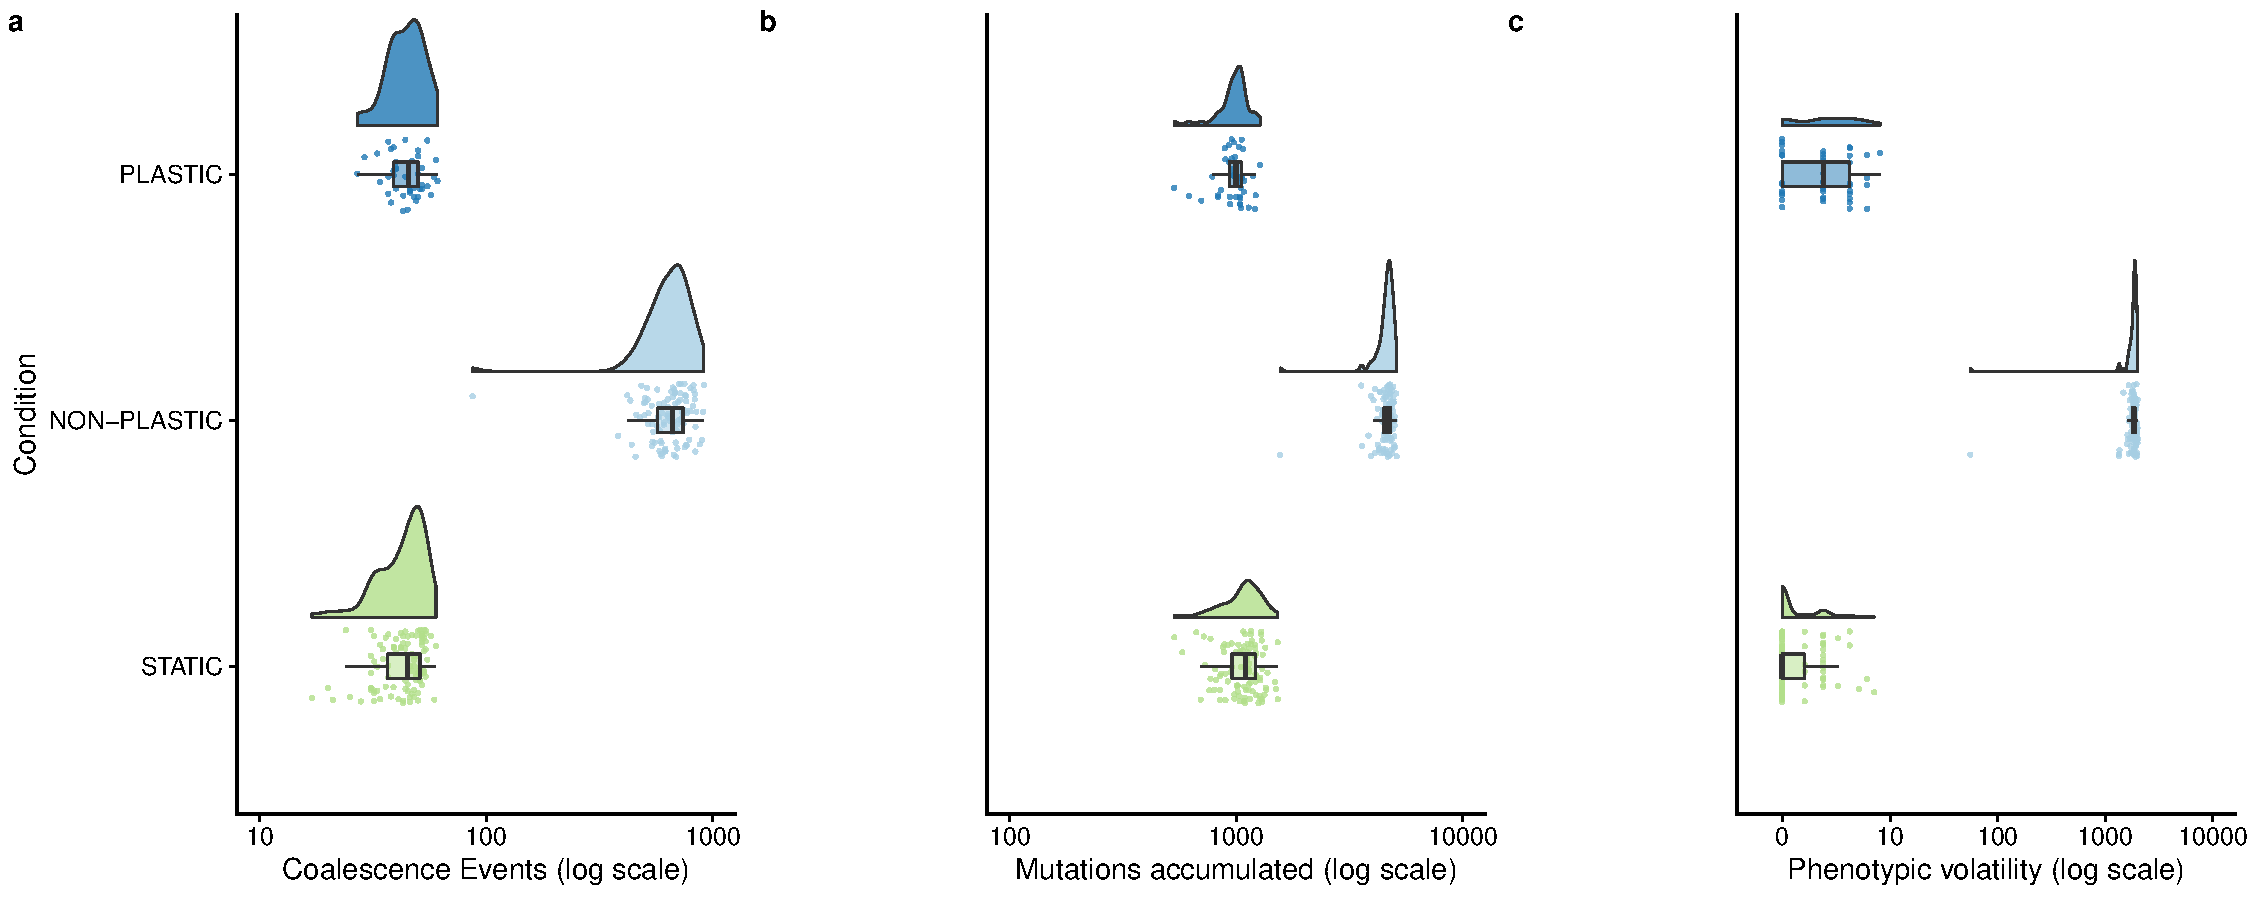
\includegraphics[width=0.9\textwidth]{media/evolutionary-dynamics.pdf}
    \caption{\small
    \textbf{todo title.}
    todo.
    }
    \label{fig:evolutionary-dynamics}
\end{figure}

%%%%%%%%%%%%%%%%%%%%%%%%%%%%%%%%%
% Results to report (2021-02-08 experiment)
% ----- GENERATIONS -----
% - average generations elapsed (of a population)
%   - NON-PLASTIC (median: 41768.65) > PLASTIC (median: 31697.65) > STATIC (median: 30839.75)
% 
% ----- SWEEPS -----
% - coalescence events (total)
%   - NON-PLASTIC (median: 663.5) > ( PLASTIC (median: 45.5) ~~ STATIC (median: 45) )
% - Average number of generations between coalescence events (gens / sweeps)
%   - ( PLASTIC (median: 685.001780758557) ~~ STATIC (median: 693.676265008576) ) > NON-PLASTIC (median: 62.0184902295191) 
% 
% ----- PHENOTYPIC VOLATILITY -----
% - phenotypic volatility (total)
%   - i.e., total number of times phenotypes change along lineages
%   - NON-PLASTIC (median: 1868) > PLASTIC (median: 2) > STATIC (median: 0)
% - phenotypic volatility / lineage length
%   - i.e., how often do genomic changes reflect changes in phenotype? 
%   - NON-PLASTIC (median: 0.437) > PLASTIC (median: 0.0022) > STATIC (median: 0)
% - phenotypic volatility / generations
%   - i.e., per-offspring rate of phenotypic changes
%   - NON-PLASTIC (median: 0.0447) > PLASTIC (median: 6.33e-05) > STATIC (median: 0)
% 
% ----- MUTATION ACCUMULATION -----
% - mutation accumulation (total)
%   - NON-PLASTIC (median: 4657.5) > STATIC (median: 1100) > PLASTIC (median: 998.5)
% - mutation accumulation / lineage length
%   - NON-PLASTIC (median: 1.10048311715591) > STATIC (median: 1.03794597464116) > PLASTIC (median: 1.0328599144651) 
% - mutation accumulation / generation
%   - NON-PLASTIC (median: 0.11) > STATIC (median: 0.0368) > PLASTIC (median: 0.0319) 
% 
% ----- MUTATIONAL EFFECTS -----
% - fraction of mutational steps that alter (aggregate) phenotype
%   - NON-PLASTIC (mean: 0.434007, CI [0.4242,  0.4406]) > PLASTIC (mean: 0.002717008, 0.0020,  0.0035) > STATIC (mean: 0.0006788834, CI [0.0004,  0.0009])
% - fraction of phenotype-altering mutation steps that alter unexpressed phenotype (PLASTIC condition only)
%   - mean: 0.8247126 CI [0.7443,  0.8994]
% - fraction of mutations that affect unexpressed phenotype that are deleterious (PLASTIC only)
%   - mean: 0.5172414 CI [0.4402,  0.5977]
% - fraction of mutations that affect unexpressed phenotype that are beneficial (PLASTIC only)
%   - mean: 0.4827586 CI [0.4046,  0.5598]
%%%%%%%%%%%%%%%%%%%%%%%%%%%%%%%%%

% -- Magnitude of evolutionary change --
%  - Selective sweeps
%  - Mutation accumulation
%  - Phenotypic volatility
%  - Number of generations elapsed
Adaptive phenotypic plasticity evolved in \evolutionaryChangeRatePlasticReps\ of \evolutionaryChangeRateReplicates\ replicates from the PLASTIC treatment during phase one of Experiment I; we used this more limited group to seed the \evolutionaryChangeRatePlasticReps\ phase-two PLASTIC replicates.
Figure [x] gives the number of coalescence events, mutation accumulation, and phenotypic volatility for PLASTIC, NON-PLASTIC, and STATIC treatments.
According to each of these metrics, NON-PLASTIC populations experienced a larger magnitude of evolutionary change than either PLASTIC or STATIC populations.
Specifically, we observed significantly more coalescence events in NON-PLASTIC populations than in PLASTIC or STATIC populations [stats].
NON-PLASTIC lineages had significantly higher mutation accumulation and phenotypic volatility than PLASTIC or STATIC lineages [stats].
Additionally, we found that significantly more generations of evolution elapsed in NON-PLASTIC populations than in PLASTIC or STATIC populations [stats]; that is, NON-PLASTIC populations exhibited a significantly higher rate of generational turnover ([data - mean, +- std dev]) than PLASTIC ([data - mean, +- stddev]) or STATIC ([data - mean, +- stddev]) populations.

% -- Rate of evolutionary change --
%   - Rate of sweeps => (generations per sweep)
%   - genotypic fidelity => frequency that offspring's genotype is identical to parent genotype (lineage length / number generations)
%   - phenotypic fidelity => frequency that an offspring's phenotype is same as parent's phenotype (phenotypic volatility / number of generations)
Next, we examined the \textit{rates} of evolutionary change across treatments to determine if the larger magnitude of evolutionary change in NON-PLASTIC populations is due to the number of additional generations elapsed during the experiment.
Specifically, we calculated the average number of generations between coalescence events as well as both genotypic fidelity and phenotypic fidelity (i.e., the frequency that an offspring's genotype or phenotype is identical to that of its parent along the dominant lineage).
We found that significantly fewer generations elapse between coalescence events in NON-PLASTIC populations than in either PLASTIC or STATIC populations [stats].
We also observed that NON-PLASTIC lineages had significantly lower genotypic and phenotypic fidelity than either PLASTIC or STATIC lineages [stats]; that is, offspring along NON-PLASTIC lineages more frequently differed genotypically and phenotypically than offspring along either PLASTIC or STATIC lineages.
Thus, our results indicate that NON-PLASTIC populations experienced both a greater magnitude of evolutionary change and a higher frequency of evolutionary change than either PLASTIC or STATIC populations.

% -- mutations affect phenotypes --
%   - fraction of mutational steps that alter (aggregate) phenotype
%   - fraction of phenotype-altering mutation steps that alter unexpressed phenotype (PLASTIC condition only)
%   - fraction of mutations that affect unexpressed phenotype that are deleterious (PLASTIC only)
%   - fraction of mutations that affect unexpressed phenotype that are beneficial (PLASTIC only)
% @AML: TODO - update with mutational stability
%   - IDEA: Terms for over 30 years working with digital evolution
We measured the fraction of mutated offspring along these lineages with a different phenotype than their parent.
For lineages evolved in fluctuating environments, we evaluated mutants under both environmental conditions and counted all changes in the \textit{aggregate} task profile.
Consistent with previous results, we found that mutated offspring along NON-PLASTIC lineages exhibit more frequent phenotypic changes from their parent than mutated offspring from either PLASTIC or STATIC lineages [stats].
% medians: NON-PLASTIC 0.437583018324547, PLASTIC 0.00224941742616098, STATIC 0
While mutational stability for PLASTIC and STATIC lineages is higher than for those from NON-PLASTIC lineages, we found that STATIC lineages exhibit a small, but significant, difference in mutational stability relative to PLASTIC lineages [stats]. 
Across all PLASTIC lineages, we found that over 80\% ([data]) of changes to task profiles occur in phenotypic traits that are expressed only in the off environment (i.e., as cryptic variation).
Approximately 52\% ([data]) of this cryptic variation degraded tasks that would have been needed in the off environment, and the remaining $\sim$48\% ([data]) were compensatory mutations; that is, they restored tasks before the environment changed.
% @AML: todo - put raw numbers in for percentages

% -- in general, PLASTIC and STATIC more similar than NON-PLASTIC --
In general, the evolution of adaptive plasticity stabilized PLASTIC treatment populations against environmental fluctuations, and their evolutionary dynamics more closely resembled those of populations evolving in a static environment.
We observed no significant difference in coalescence events in PLASTIC and STATIC populations.
We did, however, observe that, relative to STATIC populations, PLASTIC populations had more elapsed generations [significant, stats], mutation accumulation [stats], and phenotypic volatility [stats]; though these differences were statistically significant, they were not substantial.

% -- genetic architectures --
[todo - genetic architecture results]

\vspace{0.5cm}
\subsection{The evolution of novel traits}

%%%%%%%%%%%%%%%%%%%%%%%%%%%%%%%%%
% Results to report (2021-01-31)
% - Number of plastic replicates
% - Final dominant genotype # novel traits
%   - non-plastic < (plastic == static)
% - Final population (1% threshold): 
%   - non-plastic < plastic < static
% - Final population (1% threshold) discovered:
%   - non-plastic > (plastic ~~ static)
% - Lineage tasks discovered
%   - non-plastic > static ~>(nosig) plastic
% - Lineage tasks discovered / step
%   - (static ~~ plastic) > non-plastic 
% - Lineage tasks lost
%   - non-plastic > static > plastic
% - Lineage tasks lost / step
%   - non-plastic > static > plastic

% - tasks discovered per generation(?)
%   - NON-PLASTIC [0.00014358046266055] ~~ STATIC [0.00015363220504867] > PLASTIC [0.000117695011124939]
% - tasks lost per generation(?)
%   - NON-PLASTIC [0.0022026054610079] > STATIC [0.000161396283669756] > PLASTIC [6.25141973661864e-05]
%%%%%%%%%%%%%%%%%%%%%%%%%%%%%%%%%

\begin{figure}[h!]
    \centering
    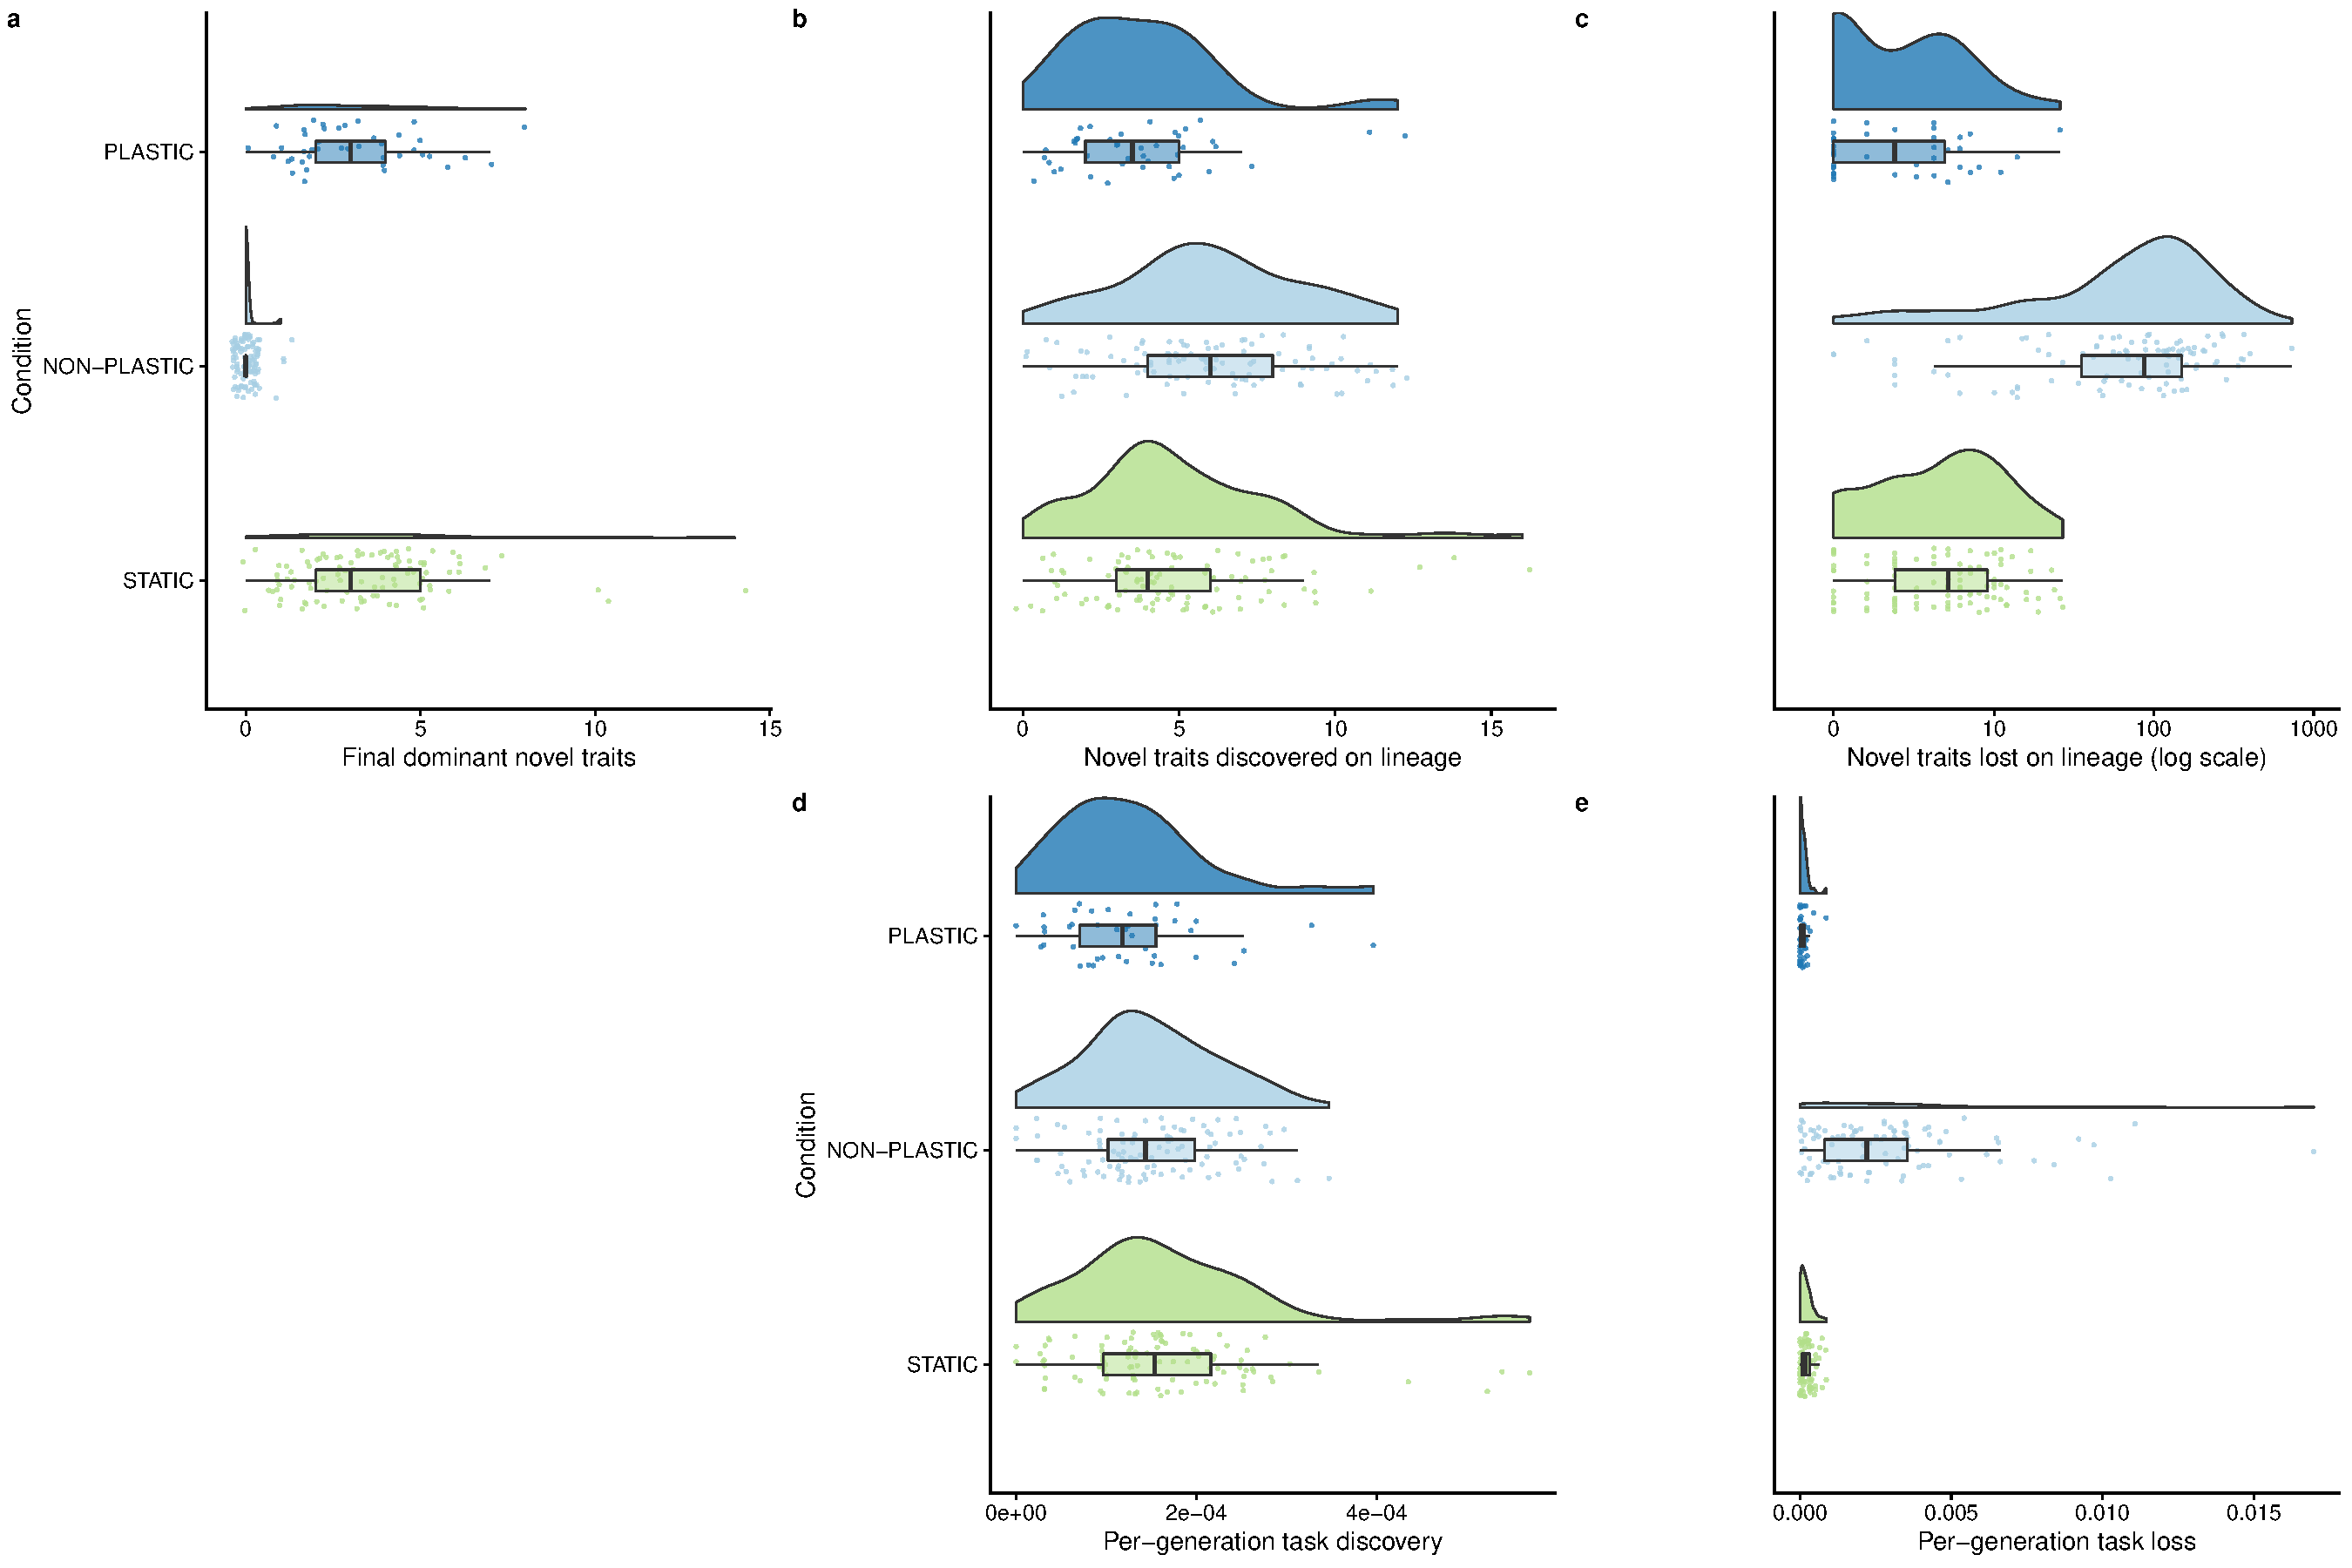
\includegraphics[width=0.9\textwidth]{media/complex-traits-panel.pdf}
    \caption{\small
    \textbf{todo title.}
    todo.
    }
    \label{fig:complex-traits}
\end{figure}

% - Magnitude of exploration/exploitation -
%   - task performance
%   - task discovery
%   - task loss
Adaptive phenotypic plasticity evolved in \novelTraitsPlasticReps\ of \novelTraitsReplicates\ replicates from the PLASTIC treatment during phase one of Experiment II; we used this more limited group to seed the \novelTraitsPlasticReps\ phase-two PLASTIC replicates.
Figure [x] shows the task discovery, task performance, and task loss for PLASTIC, NON-PLASTIC, and STATIC treatments.
We found that both PLASTIC and STATIC populations have significantly higher task performance at the end of the experiment than NON-PLASTIC populations [stats].
This, however, was not due to PLASTIC and STATIC lineages exploring a larger breadth of the fitness landscape, as NON-PLASTIC lineages had significantly higher task discovery than either PLASTIC or STATIC lineages [stats].
Indeed, we found that NON-PLASTIC lineages exhibited significantly more task loss than either PLASTIC or STATIC lineages [stats], as NON-PLASTIC lineages repeatedly failed to retain novel tasks.

% - Rates of exploration/exploitation -
%  - tasks discovered per generation(?)
%  - tasks lost per generation(?)
As noted in our evolutionary change results, a larger number of generations elapsed in NON-PLASTIC populations than in PLASTIC or STATIC populations during our experiment.
As such, we examined the \textit{rates} of task loss and task discovery: are NON-PLASTIC lineages discovering and losing novel tasks more frequently than PLASTIC or STATIC lineages?
We computed the per-generation rate of task discovery along dominant lineages and the per-generation rate of task loss along those same lineages.
We found no significant difference in per-generation task discovery between NON-PLASTIC and STATIC lineages [stats], but we did find that PLASTIC lineages had a lower per-generation task discovery rate than NON-PLASTIC or STATIC lineages [stats].
% small, but significant, per-generation task discovery rate than NON-PLASTIC or STATIC lineages [stats].
We found that NON-PLASTIC lineages had a significantly higher per-generation rate of task loss than either PLASTIC or STATIC lineages [stats], while PLASTIC lineages had a small but significantly lower per-generation rate of task loss than STATIC lineages [stats].
We cannot reject the possibility that the larger magnitude of task discovery in NON-PLASTIC lineages was driven by a larger number of elapsed generations.
Indeed, we found that NON-PLASTIC lineages repeatedly gained and failed to retain novel tasks during the experiment, and the final evolved genotypes performed fewer overall tasks.

% - Characterizing trait loss -
%   - fraction of novel trait loss co-occuring with change in base trait profile
%   - reporting overall aggregate vs. comparing distributions of fractions (among lineages that have trait loss)
% We found NON-PLASTIC lineages had sig higher fractions of task loss co-occurrence than PLASTIC and STATIC lineages [stats].
Next, we examined the frequency at which novel task loss along lineages co-occurred with base task loss (i.e., loss of any of the original six tasks).
Across all NON-PLASTIC dominant lineages, over 97\% (10998 out of 11229) of instances of novel task loss co-occurred with a simultaneous change in base task profile.
In contrast, across all PLASTIC and STATIC dominant lineages, we observed that approximately 20\% (29 out of 142) and 2\% (13 out of 631), respectively, of instances of novel task loss co-occurred with a simultaneous change in base task profile. 

\vspace{0.5cm}
\subsection{Deleterious hitchhiking}

% --@Charles editing bookmark--

%%%%%%
% 2021-02-05 - Results
% - Number of offspring on lineage where hitchhiker instruction execution increases (i.e., instances of hitchhiking)
%   - PLASTIC ~~ STATIC < NON-PLASTIC
% - Hitchhiker instruction increases / offspring on lineage
%   - PLASTIC ~~ STATIC < NON-PLASTIC
% - What fraction of mutations that increase hitchhiker instruction execution co-occur with base trait changes?
%   - NON-PLASTIC > PLASTIC ~~ STATIC
% - What about unexpressed vs expressed trait changes in plastic populations? (plastic only)
%   - Not much hitchhiking. Did not find evidence that hitchiking occurring as cryptic variation in unexpressed phenotype.
%%%%%%

% -- Instruction execution by final dominant & along lineage --
%    +
% -- Number of instructions executed per genotype --
% examining the number of times a \code{poison} instruction is executed by each genotype along the dominant lineage (including the final dominant genotype).
Adaptive phenotypic plasticity evolved in \deleteriousHitchhikingPlasticReps\ of \deleteriousHitchhikingReplicates\ replicates from the PLASTIC treatment during phase one of Experiment III; we used this more limited group to seed the \deleteriousHitchhikingPlasticReps\ phase-two PLASTIC replicates.
% Figure [x] shows the [whatever we decide] for PLASTIC, NON-PLASTIC, and STATIC treatments.
At the end of our experiment, no dominant genotypes evolved in PLASTIC or STATIC treatments expressed the \code{poison} instruction under any environmental condition; however, the dominant genotype from 14 replicates of the NON-PLASTIC treatment did express the \code{poison} instruction at least once (statistically significant, [stats]).
%The minimal instances of \code{poison} execution in dominant organisms is expected given that each execution is a 10\% reduction in metabolic rate.
The \code{poison} execution in dominant organisms is expected to be kept minimal given that each execution is a 10\% reduction in metabolic rate.


% - total offspring with increases -
Figure [x] shows the [prevalence of poison instructions in final dominant genotypes and along dominant linages] for all treatments.
%We found that the number of offspring on NON-PLASTIC lineages where \code{poison} instruction execution increases was significantly higher than that of PLASTIC or STATIC lineages [stats]; we found no significant difference in \code{poison} execution along dominant lineages between PLASTIC and STATIC lineages.
We found that NON-PLASTIC lineages had significantly more organisms that executed the \code{poison} instruction more often than their parent as compared to PLASTIC or STATIC lineages [stats]; we found no significant difference in \code{poison} execution along dominant lineages between PLASTIC and STATIC lineages.
%These numbers remain significant when normalized by number of generations ([stats]).
These significance patterns do not qualitatively change when normalized by number of generations ([stats]).

% - increases per offspring -
% We also found that the per-generation number of \code{poison} execution increases along the lineage was significantly higher in NON-PLASTIC lineages than in PLASTIC or STATIC lineages [stats], and we found no significant difference between PLASTIC and STATIC lineages.

% -- When/where does hitchhiking take place? --
Next, we examined the frequency that mutations that increase \code{poison} execution co-occur with mutations that change the base task profile of offspring along dominant lineages across treatments.
Across all NON-PLASTIC dominant lineages, we found that approximately 49\% (956 out of 1916) mutations that increased \code{poison} execution co-occurred with mutations that changed the base task profile; we observed zero instances of co-occurrence in PLASTIC and STATIC lineages.
Additionally, we did not find evidence that mutations that increased \code{poison} execution occurred as cryptic variation in PLASTIC lineages.



